\documentclass[letterpaper]{article}
\title{CSE 550 Introduction to Systems Research \\ Problem Set 2}

\usepackage{balance}  % to better equalize the last page
\usepackage{graphicx}
\usepackage{times}    % comment if you want LaTeX's default font
\usepackage{url}      % llt: nicely formatted URLs
\usepackage{graphicx}
\usepackage{tabularx}
\usepackage{float}
\usepackage{color}
\usepackage{url}
\usepackage[noend]{algpseudocode}
\usepackage{algorithm}
\usepackage{verbatim}
\usepackage{mathtools}
\usepackage{caption}
\usepackage{subcaption}
%\usepackage{amsmath}
\let\proof\relax
\let\endproof\relax
\usepackage{amsthm}
\usepackage{thmtools}
\usepackage{xspace}
\usepackage{multirow}
\newcommand{\field}[1]{\mathbb{#1}} 
\newcommand{\hide}[1]{#1}
\newcommand{\pd}[2]{\frac{\partial #1}{\partial #2}}
\providecommand{\m}[1]{\mathbf{#1}}
\providecommand{\norm}[1]{\left\|#1\right\|}
\providecommand{\sign}[1]{\text{sign}\left(#1\right)}
\DeclareMathOperator*{\argmin}{arg\,min}
\providecommand{\what}{\m{\hat{w}}}

\begin{document}
\author{Marco Tulio Correia Ribeiro, Shrainik Jain\\ 1323300, 1323338}
\maketitle

\section{Implementation}
The base system is a set of Nodes, each running a PaxosHandler instance and a Broker which acts as a middleware to interpret client requests. All the communication is done using the Apache Thrift Framework. Any client can contact Broker at any node, with a command of the form {\em Lock mutexId clientId} or {\em Unlock mutexNo clientId}. The Broker relays the commands to the PaxosHandler in the same Node. \\

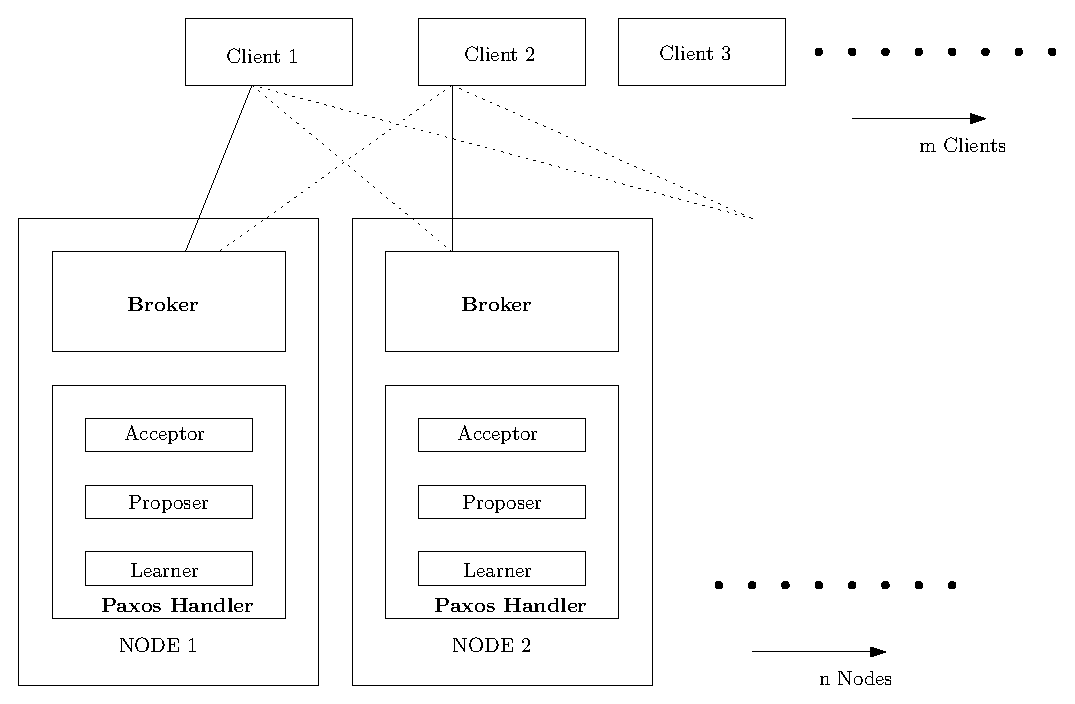
\includegraphics[width = 4.5in, keepaspectratio]{Architecture.eps}\\

PaxosHandler implements {\em leader Paxos}. Upon receiving a run command request, each node checks if it is the leader, if true, it starts an instance of Paxos with the value as the command recieved. If the node recieving the client request is not the leader, it asks the leader to run the newer command.\\
When the leader goes down, the nodes cannot contact the leader to run the command, and thus start a round for Election of new leader, and then send the command to the newer leader.\\
To ensure that the 2 nodes don't compete as leaders (in the case where a leader goes down, and then comes back up after some other node has been elected as the leader), each node maintains a list a promised proposals indexed by instance number. Electnewleader ensures that this list is updated such that the older leader will always sees a proposal number greater than it proposes When this happens the code is structured such that the node realizes that it is not the leader anymore, and figures out who the new leader is (Figuring out the new leader is easy enough since we maintain a convention of proposal numbers to end with the leader id).

\section{Assumptions}
\begin{itemize}
\item For the sake of the assignment, we assume that the number of nodes is less than 1000.
\item Reconfiguration and recovery is not supported.
\item Client does the error handling itself. i.e. if the there is an error in the communication between client and a node, the client implements the retry/ignore logic.
\end{itemize}
\section{Running the code}
To ease the starting of the servers and brokers, we are submitting a few scripts.
\begin{itemize}
\item {\em start\_nodes.py}: Starts as many nodes (broker and paxos handlers) as given via argument. Usage:
\begin{verbatim}
start_nodes.py -l NUM_LOCKS -n NUM_NODES
\end{verbatim}
This will start a bunch of nodes as servers running on different ports on the localhost. And will also output the port numbers for the broker and paxoshandler on each node. After this you can just run the following commands on the client:
\begin{verbatim}
Broker-remote [-h host[:port]] Lock mutexNo ClientId
\end{verbatim}
Or
\begin{verbatim}
Broker-remote [-h host[:port]] Unlock mutexNo ClientId
\end{verbatim}

\item {\em test-failed-message.sh}: Script to simulate failed messages. (Automatically calls start\_nodes.py)
\item {\em test-kill-leader.sh}: Script to kill a leader and see if the Paxos nodes are still working. (Automatically calls start\_nodes.py)
\item {\em test-kill-2-leaders.sh}: Script to kill one leader after another to see if the Paxos nodes are still working. (Automatically calls start\_nodes.py)

\end{itemize}
\section{Issues}
\emph{Should be talk about locking issues here?}


\end{document}